\documentclass[a4paper,12pt]{article}
\usepackage[utf8]{inputenc}
\usepackage[cm,empty]{fullpage}
\usepackage[T2A]{fontenc}
\usepackage[english, russian]{babel}
\usepackage{amssymb,amsmath,amsxtra,amsthm}
\usepackage{proof}
\usepackage[pdftex]{graphicx}
\usepackage{wrapfig}
\usepackage{braket}
\usepackage{xcolor}
\usepackage{enumitem}

\usepackage[left=2cm,right=2cm,
    top=1cm,bottom=1cm,bindingoffset=0cm]{geometry}

\renewcommand{\leq}{\leqslant}
\renewcommand{\geq}{\geqslant}


\newcommand{\iiff}{\Longleftrightarrow}
\renewcommand{\iff}{\Leftrightarrow}
\newcommand{\nothing}{\varnothing}

\newtheorem*{rem}{Замечание}

\newcommand{\NN}{\mathbb{N}}
\newcommand{\ZZ}{\mathbb{Z}}
\newcommand{\Q}{\mathbb{Q}}
\newcommand{\A}{\mathbb{A}}
\newcommand{\R}{\mathbb{R}}
\renewcommand{\C}{\mathbb{C}}

\renewcommand{\phi}{\varphi}
\newcommand{\eps}{\varepsilon}

\makeatletter
\newcommand*{\rom}[1]{\expandafter\@slowromancap\romannumeral #1@}
\makeatother

\newcounter{z}


\newcommand{\zs}{\refstepcounter{z}\vskip 10pt\par\noindent
\fbox{\textbf{12.\arabic{z}}} }

\newcommand{\z}{\refstepcounter{z}\vskip 20pt\noindent
\fbox{\textbf{\arabic{z}}} }

\renewcommand{\date}{{\bf 27 апреля 2021}} 

\newcommand{\dif}
{
------------------------------------------------------------------------------------------------------------------------------------------------------
}

\newcommand{\HSEhat}{
\vspace*{-0pt}
\noindent
\setcounter{z}{0}


{\bf \phantom{\date}  \large \hfill Линейная алгебра: \hfill \normalsize \date}

\vspace{5 pt}
{\bf \large \hfill  лекция 6\hfill }

\vspace{15 pt}
\centerline{ \large  Домашнее задание.}
\centerline{ \large  Кирилл Сетдеков}



\vspace*{10pt}
\setcounter{z}{0}

}

\begin{document}
\HSEhat


\begin{enumerate}

\subsection*{Задачи:}



\item Чему может быть равен определитель вещественной ортогональной $n \times n$ матрицы? (Перечислите все возможные варианты и обоснуйте, что других вариантов нет)

\vspace{5pt}

\textbf{Решение:}\\
По свойству ортогональной матрицы: $AA^T = E$\\ 
Следовательно определитель произведение самой на транспонированную равен 1 $$|AA^T| = |E|=1$$
Разложим $|AA^T|$:
$$|AA^T|=|A||A^T|=|A||A|=1$$
Заменим $|A|=x\Rightarrow x^2 =1$\\
У этого уравнения 2 решения: -1 и 1. Так как мы пришли к этому из свойств определителя и определения ортогональной матрицы, то это единственные варианты.
\textbf{Ответ: Возможные значения определителя $-1,1$}


\item Диагонализуйте следующие симметрические матрицы в ортонормированном базисе (то есть получите разложение\\ $A = C D C^T$, где $C$ -- ортогональная матрица, а $D$ -- диагональная):

\vspace{5pt}


а)  
$
\begin{pmatrix}
{2}&{1}\\
{1}&{2}\\
\end{pmatrix}
$


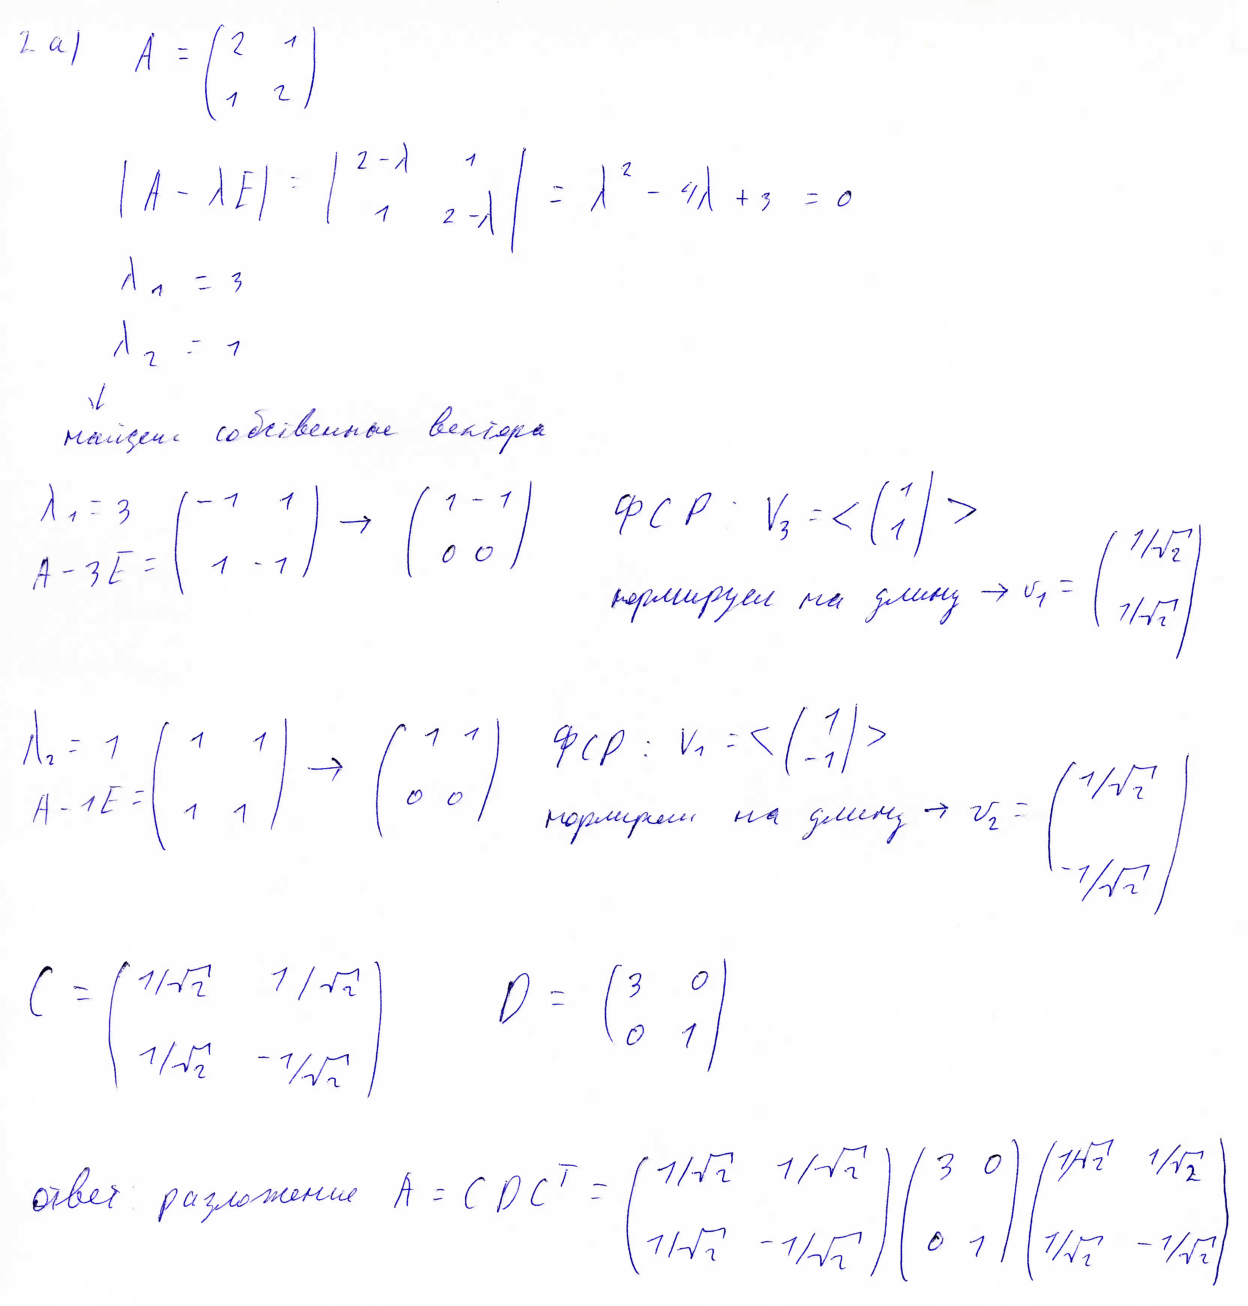
\includegraphics[width=\textwidth]{img/img200.pdf}


б) 
$
\begin{pmatrix}
{0}&{0}&{1}\\
{0}&{1}&{0}\\
{1}&{0}&{0}\\
\end{pmatrix}
$


\vspace{5pt}
\textbf{Решение:}\\
$A =\begin{pmatrix}
{0}&{0}&{1}\\
{0}&{1}&{0}\\
{1}&{0}&{0}\\
\end{pmatrix}$
Найдем характеристический многочлен и его корни:\\
$|A-\lambda E|= \begin{vmatrix}
{-\lambda}&{0}&{1}\\
{0}&{1-\lambda}&{0}\\
{1}&{0}&{-\lambda}\\
\end{vmatrix}=(\lambda-1)\begin{vmatrix}
{-\lambda}&{1}\\
{1}&{-\lambda}\\
\end{vmatrix}=(\lambda-1)(\lambda^2-1)=(\lambda-1)^2(\lambda+1)=0$

Корнями будут $\lambda_{1,2} =1$ - кратности 2 и $\lambda_3 = -1$

Найдем собственные вектора:\\
$\lambda_{1,2} =1$\\
$A-E = \begin{pmatrix}
{-1}&{0}&{1}\\
{0}&{0}&{0}\\
{1}&{0}&{-1}\\
\end{pmatrix}\rightarrow\begin{pmatrix}
{-1}&{0}&{1}\\
{0}&{0}&{0}\\
{0}&{0}&{0}\\
\end{pmatrix}$ В этой матрице только 1 главная переменная, следовательно ФСР будет состоять из двух векторов. ФСР: $V_1=<\begin{pmatrix}
0\\
1\\
0
\end{pmatrix},\begin{pmatrix}
1\\
0\\
1
\end{pmatrix}>$. Они ортогональны, нормируем их на длину, чтобы получить ортонормированные вектора: $v_1 = \begin{pmatrix}
0\\
1\\
0
\end{pmatrix}$, $v_2 = \begin{pmatrix}
\frac{1}{\sqrt{2}}\\
0\\
\frac{1}{\sqrt{2}}
\end{pmatrix}$\\

Рассмотрим $\lambda_3 = -1$\\
$A+E = \begin{pmatrix}
{1}&{0}&{1}\\
{0}&{2}&{0}\\
{1}&{0}&{1}\\
\end{pmatrix}\rightarrow\begin{pmatrix}
{1}&{0}&{1}\\
{0}&{1}&{0}\\
{0}&{0}&{0}\\
\end{pmatrix}$ В этой матрице 2 главные переменные, следовательно ФСР будет состоять из одного вектора. $V_{-1}=<\begin{pmatrix}
-1\\
0\\
1
\end{pmatrix}>$. Нормируем его $\rightarrow v_3 = \begin{pmatrix}
-\frac{1}{\sqrt{2}}\\
0\\
\frac{1}{\sqrt{2}}
\end{pmatrix}$

Выпишем $C=(v_1|v_2|v_3)$ и $D$ как диагональную матрицу из соответствующих собственных значений.
$$C=\begin{pmatrix}
0&\frac{1}{\sqrt{2}}&-\frac{1}{\sqrt{2}}\\
1&0&0\\
0&\frac{1}{\sqrt{2}}&\frac{1}{\sqrt{2}}
\end{pmatrix}$$
$$D=\begin{pmatrix}
{1}&{0}&{0}\\
{0}&{1}&{0}\\
{0}&{0}&{-1}\\
\end{pmatrix}$$
\textbf{Ответ: Разложение $A = C D C^T = \begin{pmatrix}
0&\frac{1}{\sqrt{2}}&-\frac{1}{\sqrt{2}}\\
1&0&0\\
0&\frac{1}{\sqrt{2}}&\frac{1}{\sqrt{2}}
\end{pmatrix}\begin{pmatrix}
{1}&{0}&{0}\\
{0}&{1}&{0}\\
{0}&{0}&{-1}\\
\end{pmatrix}
\begin{pmatrix}
0&1&0\\
\frac{1}{\sqrt{2}}&0&\frac{1}{\sqrt{2}}\\
-\frac{1}{\sqrt{2}}&0&\frac{1}{\sqrt{2}}
\end{pmatrix}$}


\item  Пусть задана матрица:
$$A = 
\begin{pmatrix}
{13}&{14}&{4}\\
{14}&{24}&{18}\\
{4}&{18}&{29}\\
\end{pmatrix}.$$

\vspace{5pt}


а) Найдите разложение $A = C D C^T$, где $C$ -- ортогональная матрица, а $D$ -- диагональная.

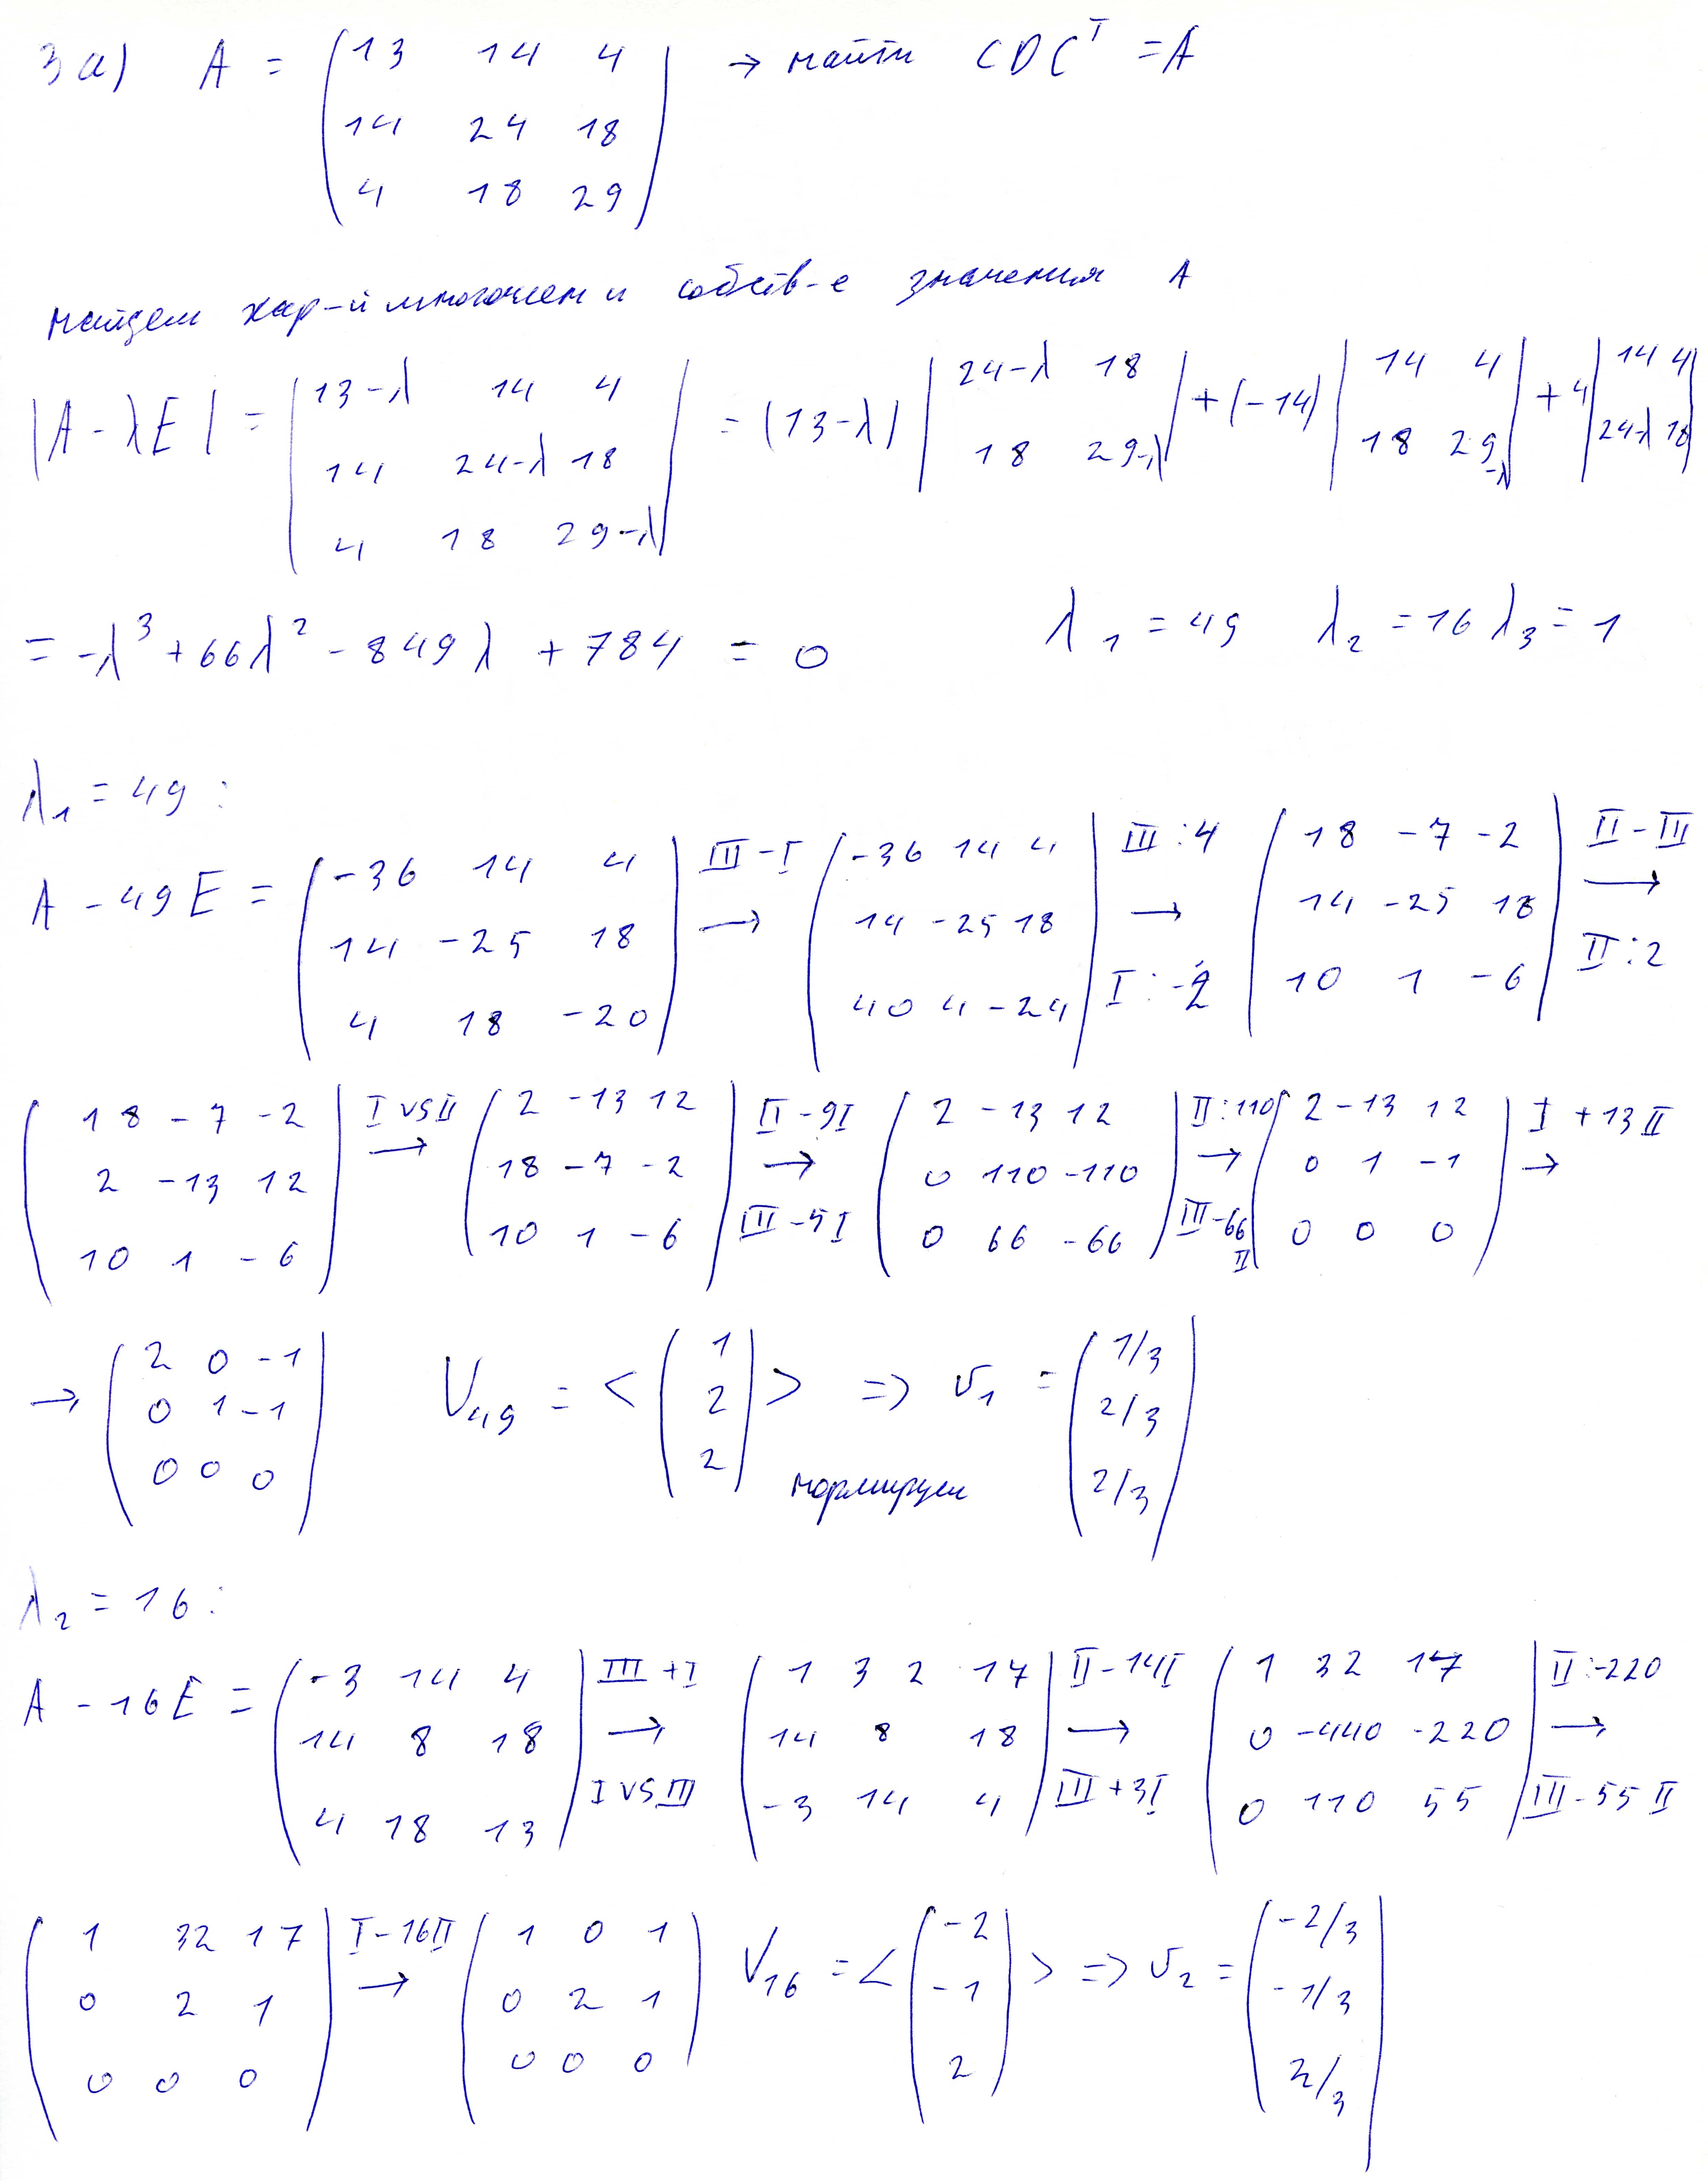
\includegraphics[width=\textwidth]{img/img201-min.jpg}
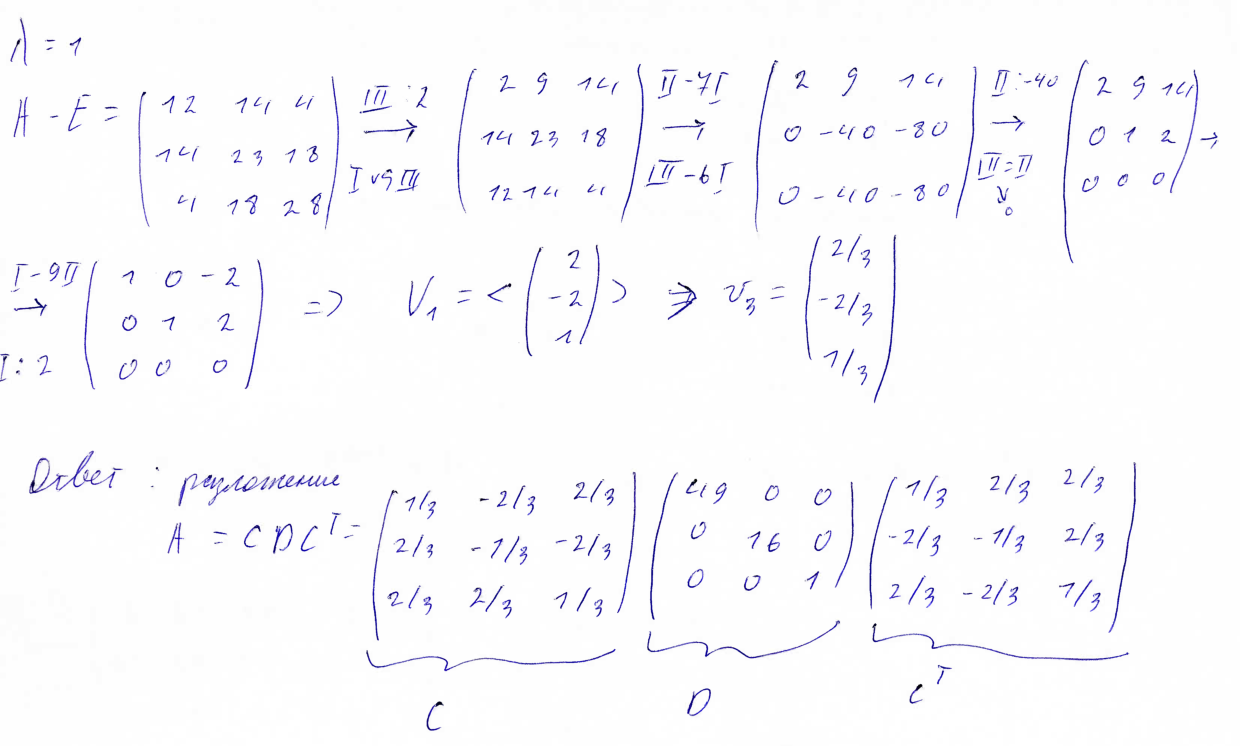
\includegraphics[width=\textwidth]{img/img202.pdf}


б) Найдите какую-нибудь симметрическую матрицу $B$ такую, что $B^2 = A$.

\vspace{5pt}
\textbf{Решение:}\\
Мы уже нашли разложение для симметричной матрицы $A = C D C^T$.
Найдем $K: K^2 = D$. Так как $D$ - диагональная матрица, то $K$ можно построить, взяв квадратный корень поэлементно из значений $D$. 
$$K = \begin{pmatrix}
7&0&0\\
0&4&0\\
0&0&1\\
\end{pmatrix}$$

Матрица $B$ такую, что $B^2 = A$ может быть найдена как $B=C K C^T$:
$$B=C K C^T=\frac{1}{3}\begin{pmatrix}
1&-2&2\\
2&-1&-2\\
2&2&1\\
\end{pmatrix}
\begin{pmatrix}
7&0&0\\
0&4&0\\
0&0&1\\
\end{pmatrix}\frac{1}{3}\begin{pmatrix}
1&2&2\\
-2&-1&2\\
2&-2&1\\
\end{pmatrix}=$$
$$=\frac{1}{9}\begin{pmatrix}
7&-8&2\\
14&-4&-2\\
14&8&1\\
\end{pmatrix}\begin{pmatrix}
1&2&2\\
-2&-1&2\\
2&-2&1\\
\end{pmatrix}=\frac{1}{9}\begin{pmatrix}
27&18&0\\
18&36&18\\
0&18&45\\
\end{pmatrix}=\begin{pmatrix}
3&2&0\\
2&4&2\\
0&2&5\\
\end{pmatrix}$$

Для проверки: $B^2=\begin{pmatrix}
3&2&0\\
2&4&2\\
0&2&5\\
\end{pmatrix}\begin{pmatrix}
3&2&0\\
2&4&2\\
0&2&5\\
\end{pmatrix}=\begin{pmatrix}
{13}&{14}&{4}\\
{14}&{24}&{18}\\
{4}&{18}&{29}\\
\end{pmatrix}=A$\\
\textbf{Ответ: Одно из возможных решений $A=B^2$: $B=\begin{pmatrix}
3&2&0\\
2&4&2\\
0&2&5\\
\end{pmatrix}$}

\item Найдите сингулярное разложение и усечённое сингулярное разложение следующих матриц:

\vspace{5pt}


а)
$
\begin{pmatrix}
{5}&{1}&{8}\\
{7}&{5}&{4}
\end{pmatrix}
$

\vspace{5pt}
\textbf{Решение:}\\
Найдем сначала сингулярное разложение.
$A = C \Lambda D^T$


$S=AA^T=\begin{pmatrix}
5&1&8\\
7&5&4
\end{pmatrix}\begin{pmatrix}
5&7\\
1&5\\
8&4
\end{pmatrix} = \begin{pmatrix}
90&72\\
72&90\\
\end{pmatrix}$

Найдем характеристический многочлен для $S$ и собственные вектора и собственные значения.
$X_S(\lambda) = \lambda^2-(tr(S)\lambda)+|S|=\lambda^2-180\lambda+2916 = (\lambda-18)(\lambda-162)$

Корни найдены как решение квадратного уравнения.\\
Рассмотрим $\lambda=162$\\
$S-162E=\begin{pmatrix}
-72&72\\
72&-72\\
\end{pmatrix} \rightarrow\begin{pmatrix}
-1&1\\
0&0\\
\end{pmatrix} $

ФСР: будет вектор, который мы сразу разделим на его длину, чтобы иметь длину 1 $v_1 = \frac{1}{\sqrt{2}}\begin{pmatrix}
1\\
1
\end{pmatrix}$

Рассмотрим $\lambda=18$\\
$S-18E=\begin{pmatrix}
72&72\\
72&72\\
\end{pmatrix} \rightarrow\begin{pmatrix}
1&1\\
0&0\\
\end{pmatrix}$

ФСР: будет вектор, который мы сразу разделим на его длину, чтобы иметь длину 1 $v_2 = \frac{1}{\sqrt{2}}\begin{pmatrix}
1\\
-1
\end{pmatrix}$


Запишем $C = (v_1|v_2)=\frac{1}{\sqrt{2}}\begin{pmatrix}
1&1\\
1&-1\\
\end{pmatrix}$\\
$\Lambda$ найдем, записав в порядке убывания квадратные корни из собственных значений $S$ по диагонали $\Lambda=\begin{pmatrix}
\sqrt{162}&0&0\\
0&\sqrt{18}&0
\end{pmatrix}=\begin{pmatrix}
9\sqrt{2}&0&0\\
0&3\sqrt{2}&0
\end{pmatrix}$

Матрица $D$ в этом задании состоит из 2 частей: $size(D_1)=(3X2), size(D_2)=(3X1)$ и $D = (D_1|D_2)$.
Найдем из условия $A = C \Lambda D^T$ сначала $D_1$.

$${\begin{pmatrix}
9\sqrt{2}&0\\
0&3\sqrt{2}
\end{pmatrix}}^{-1} C^T A = D_1^T$$

$$D_1^T={\begin{pmatrix}
\frac{\sqrt{2}}{18}&0\\
0&\frac{3\sqrt{2}}{18}
\end{pmatrix}} \frac{1}{\sqrt{2}}\begin{pmatrix}
1&1\\
1&-1\\
\end{pmatrix} \begin{pmatrix}
{5}&{1}&{8}\\
{7}&{5}&{4}
\end{pmatrix} = \frac{1}{18}{\begin{pmatrix}
1&0\\
0&3
\end{pmatrix}} \begin{pmatrix}
1&1\\
1&-1\\
\end{pmatrix} \begin{pmatrix}
{5}&{1}&{8}\\
{7}&{5}&{4}
\end{pmatrix}  $$

$$D_1^T=\frac{1}{18}\begin{pmatrix}
12&6&12\\
-6&-12&12\\
\end{pmatrix} = \begin{pmatrix}
\frac{2}{3}&\frac{1}{3}&\frac{2}{3}\\
-\frac{1}{3}&-\frac{2}{3}&\frac{2}{3}\\
\end{pmatrix}$$
Длины векторов из строк равны 1 $|D_1^T[0]|=|D_1^T[1]|=1$ и их скалярное произведение $(D_1^T[0],D_1^T[1])=0 \Rightarrow$ они уже ортонормированные.\\
Построим $D_2$ так чтобы это получился вектор, ортогональный векторам $U_1 = \begin{pmatrix}
\frac{2}{3}&\frac{1}{3}&\frac{2}{3}
\end{pmatrix}$ и  $U_2 = \begin{pmatrix}
-\frac{1}{3}&-\frac{2}{3}&\frac{2}{3}\\
\end{pmatrix}$ одновременно. Найдем его через решение методом Гаусса системы линейных уравнений относительно его координат $x,y,z$\\
$
\left(\begin{array}{ccc}  
2&1&2\\
-1&-2&2\\
\end{array}\right) \rightarrow$ прибавим к \rom{1} + \rom{2}\\

$
\left(\begin{array}{ccc}  
1&-1&4\\
-1&-2&2\\
\end{array}\right) \rightarrow$  \rom{2} + \rom{1}\\
$
\left(\begin{array}{ccc}  
1&-1&4\\
0&-3&6\\
\end{array}\right) \rightarrow$  \rom{2} :-3\\
$
\left(\begin{array}{ccc}  
1&-1&4\\
0&1&-2\\
\end{array}\right) \rightarrow$  \rom{1}+ \rom{2}\\
$
\left(\begin{array}{ccc}  
1&0&2\\
0&1&-2\\
\end{array}\right) \rightarrow$  запишем ФСР и поделим сразу вектор на его длину\\
$v_3 = \begin{pmatrix}
-2\\2\\1
\end{pmatrix} \frac{1}{3}$

Запишем ответ, используя для усеченного разложения только 2 колонки в $\Lambda$ и 2 строки в $D^T$:\\
\textbf{Ответ: SVD разложение исходной матрицы:\\ $A = \begin{pmatrix}
\frac{1}{\sqrt{2}}&\frac{1}{\sqrt{2}}\\
\frac{1}{\sqrt{2}}&-\frac{1}{\sqrt{2}}\\
\end{pmatrix} \begin{pmatrix}
9\sqrt{2}&0&0\\
0&3\sqrt{2}&0
\end{pmatrix} \begin{pmatrix}
\frac{2}{3}&\frac{1}{3}&\frac{2}{3}\\
-\frac{1}{3}&-\frac{2}{3}&\frac{2}{3}\\
-\frac{2}{3}&\frac{2}{3}&\frac{1}{3}
\end{pmatrix}$ \\
Усеченное SVD разложение:
$A = \begin{pmatrix}
\frac{1}{\sqrt{2}}&\frac{1}{\sqrt{2}}\\
\frac{1}{\sqrt{2}}&-\frac{1}{\sqrt{2}}\\
\end{pmatrix} \begin{pmatrix}
9\sqrt{2}&0\\
0&3\sqrt{2}
\end{pmatrix} \begin{pmatrix}
\frac{2}{3}&\frac{1}{3}&\frac{2}{3}\\
-\frac{1}{3}&-\frac{2}{3}&\frac{2}{3}\\
\end{pmatrix}$ }


б)
$
\begin{pmatrix}
{1}&{1}&{2}&{2}\\
{2}&{2}&{1}&{1}
\end{pmatrix}
$

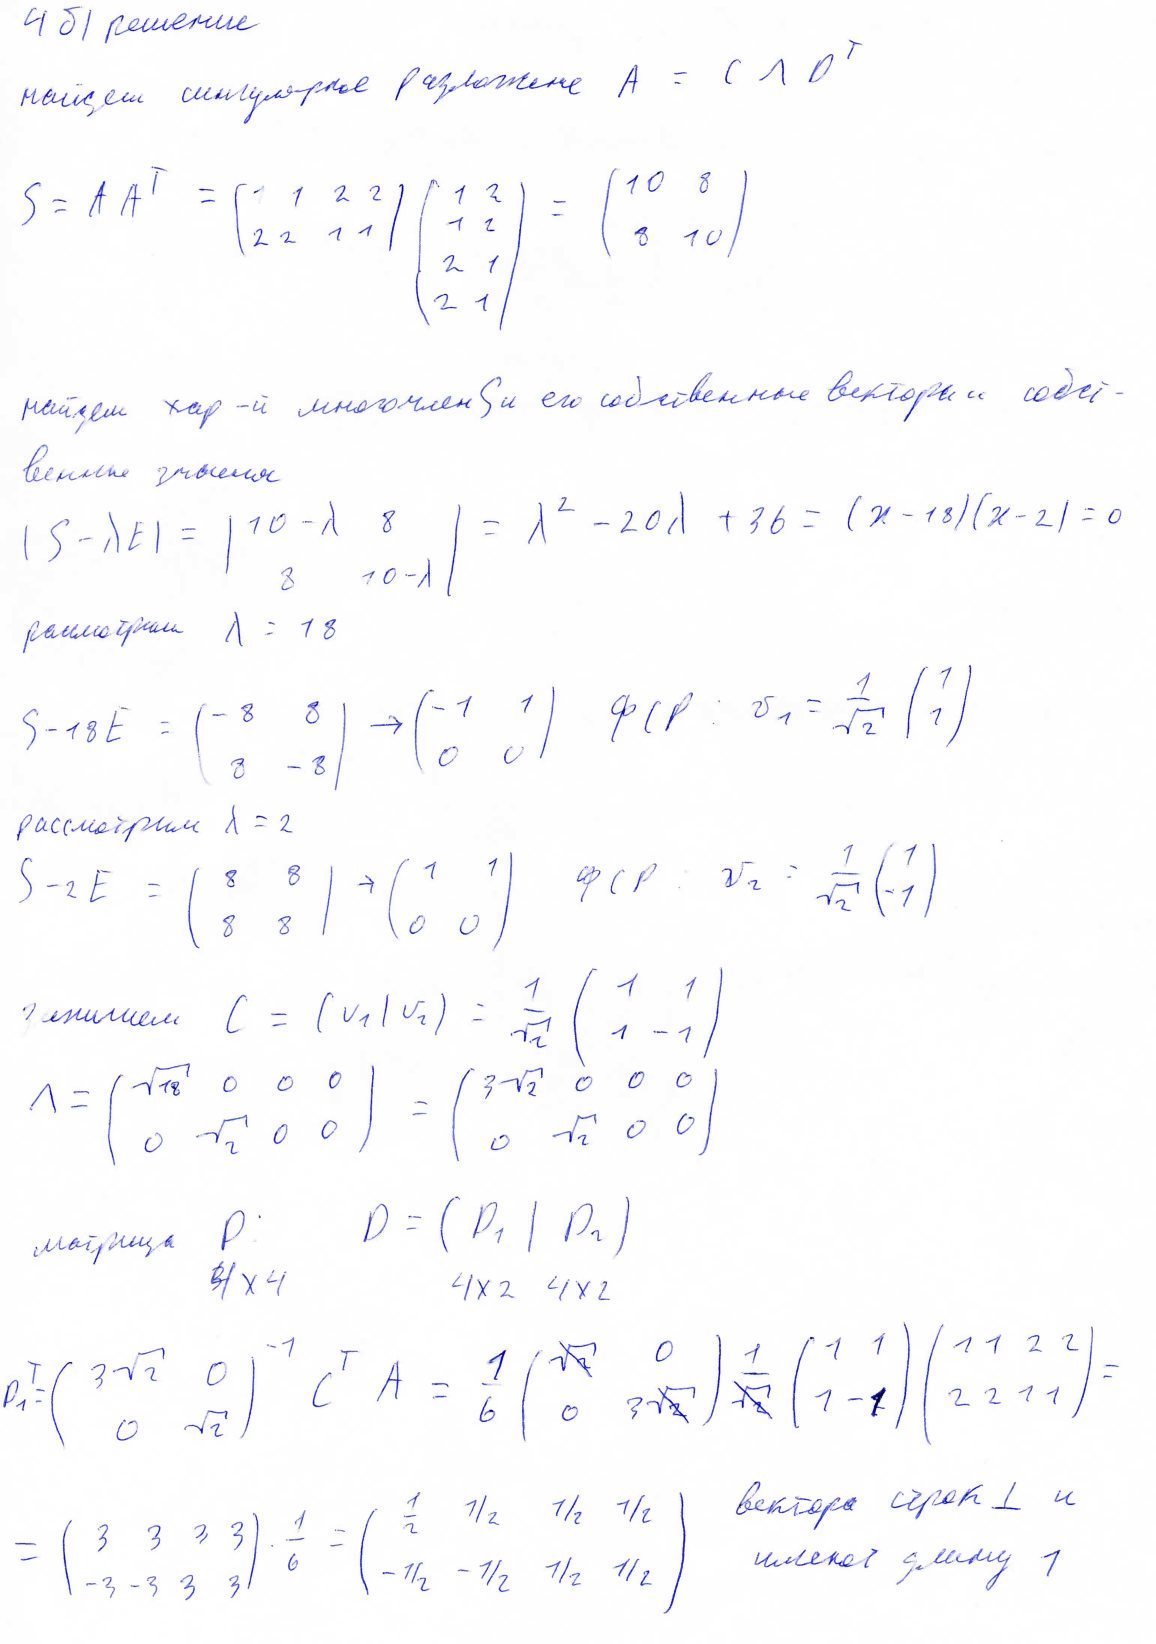
\includegraphics[width=0.9\textwidth]{img/img205.pdf}\\
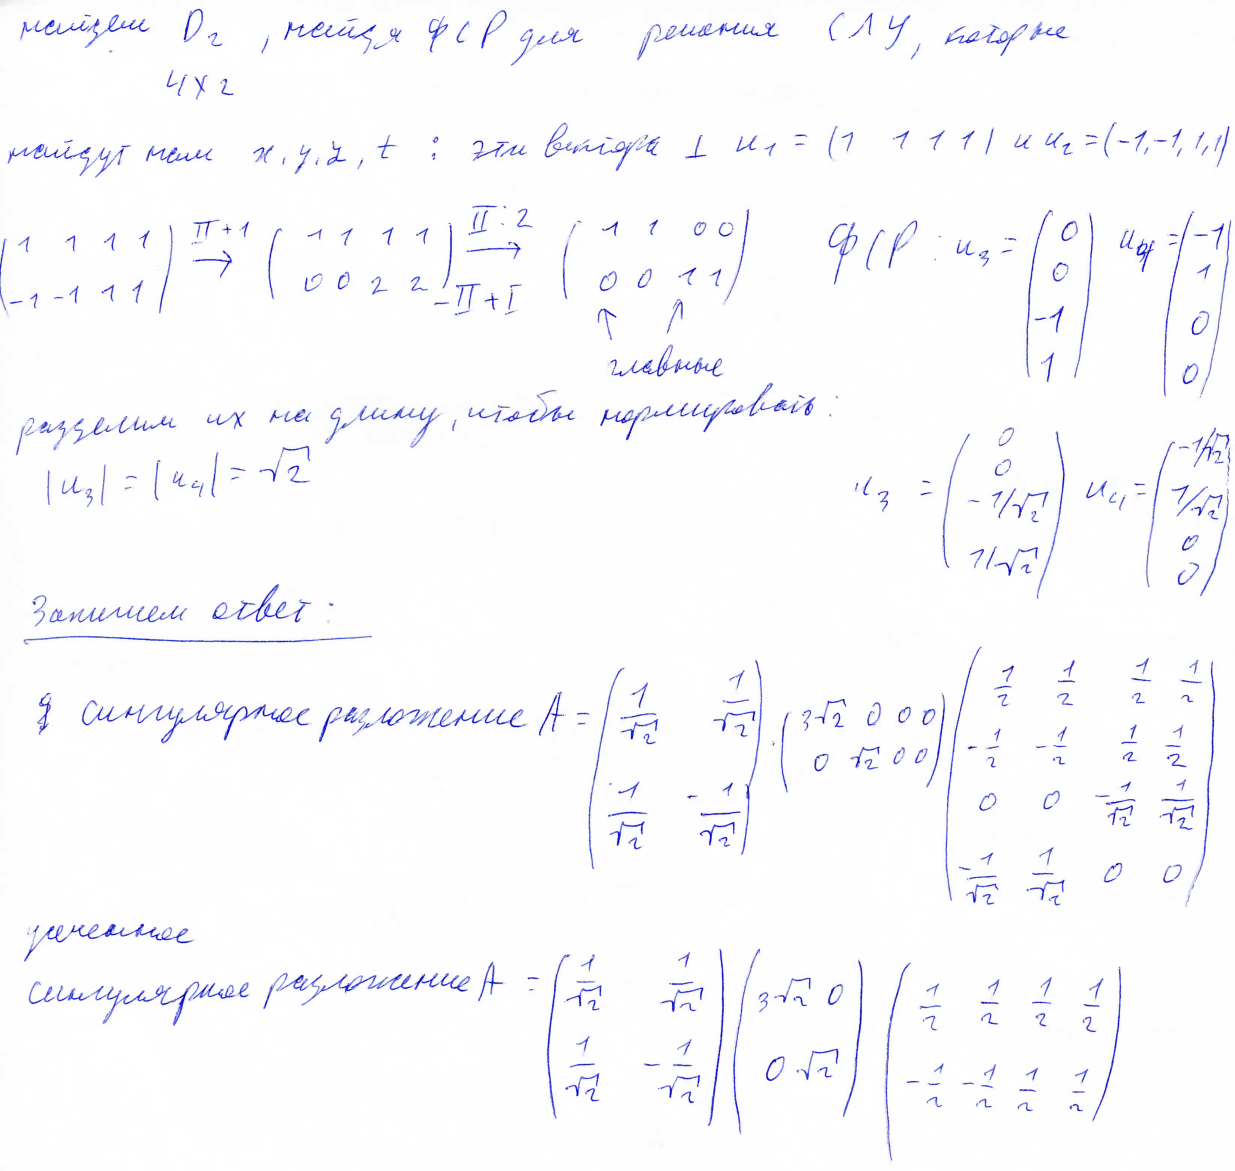
\includegraphics[width=\textwidth]{img/img206.pdf}

в) 
$
\begin{pmatrix}
7 & 1 & 2\\
5 & 5 & -2\\
3 & 3 & 6\\
-1 & -7 & -2
\end{pmatrix}
$

\vspace{5pt}
\textbf{Решение:}\\
Найдем сначала сингулярное разложение.
$A = C \Lambda D^T$
Так как в нашей исходной матрице столбцов меньше, чем строк, то возьмем $B=A^T$, пойдем по алгоритму для нахождения разложения $B=C\Lambda D^T$, а потом запишем $A=D {\Lambda}^T C^T$ для исходной матрицы.
$$S = B B^T = \begin{pmatrix}
84&48&24\\
48&84&24\\
24&24&48
\end{pmatrix}=12\begin{pmatrix}
7&4&2\\
4&7&2\\
2&2&4
\end{pmatrix}$$
Найдем характеристический многочлен для $S/12$ и собственные вектора и собственные значения $\lambda_i^{'}$. Чтобы получить собственные значения для исходной $S$, умножим $12 \cdot  \lambda_i^{'}=\lambda_i$, а собственные вектора для $S/12$ и $S$ будут совпадать.
$X_S(\lambda) = |S/12-\lambda^{'} E|= \begin{vmatrix} 
7-\lambda^{'}&4&2\\
4&7-\lambda^{'}&2\\
2&2&4-\lambda^{'}
\end{vmatrix}=-{\lambda^{'}}^3+18{\lambda^{'}}^2-81{\lambda^{'}}+108=-({\lambda^{'}}-12)({\lambda^{'}}-3)^2=0$

$\lambda_1^{'}=12, \lambda_1=144$\\
$\lambda_{2,3}^{'}=3, \lambda_{2,3}=36$\\

Рассмотрим $\lambda_1^{'}=12, \lambda_1=144$\\
$S/12-12E=\begin{pmatrix}
-5&4&2\\
4&-5&2\\
2&2&-8\\
\end{pmatrix} \rightarrow$ \rom{1} +  \rom{2}, \rom{2} $\cdot(-1)$ 
$\begin{pmatrix}
1&1&-4\\
4&-5&2\\
2&2&-8\\
\end{pmatrix} \rightarrow$ \rom{2} -4  \rom{1}, \rom{4} -2\rom{1}  
$\begin{pmatrix}
1&1&-4\\
0&-9&18\\
0&0&0\\
\end{pmatrix} \rightarrow$ \rom{2} /-9 
$\begin{pmatrix}
1&1&-4\\
0&1&-2\\
0&0&0\\
\end{pmatrix} \rightarrow$ \rom{1} - \rom{2} 
$\begin{pmatrix}
1&0&-2\\
0&1&-2\\
0&0&0\\
\end{pmatrix} \Rightarrow$ 1 и 2 столбцы - главные, запишем ФСР и сразу нормализуем вектор $v_1 = \frac{1}{3}\begin{pmatrix}
2\\
2\\
1
\end{pmatrix}$

Рассмотрим $\lambda_{2,3}^{'}=3, \lambda_{2,3}=36$\\
$S/12-3E=\begin{pmatrix}
4&4&2\\
4&4&2\\
2&2&1\\
\end{pmatrix} \rightarrow\begin{pmatrix}
2&2&1\\
0&0&0\\
0&0&0\\
\end{pmatrix}$ тут только 1 главный столбец.\\
ФСР: $<(v_2 =\begin{pmatrix}
-1\\
1\\
0
\end{pmatrix},v_3 =\begin{pmatrix}
-1/2\\
0\\
1
\end{pmatrix})>$

$v_2, v_3$ не ортогональны, так как $(v_2, v_3)\neq0 \Rightarrow$ проведем ортогонализацию Грамма-Шмидта для $v_2, v_3$:\\
Возьмем $u_2 = v_2 = \begin{pmatrix}
-1\\
1\\
0
\end{pmatrix}$ так как он ортогонален $v_1$. Найдем $u_3$:
$$u_3=v_3-{pr}_{u_2}v_3=v_3-\frac{(u_2,v_3)}{(u_2,u_2)}\cdot u_2=\begin{pmatrix}
-1/2\\
0\\
1
\end{pmatrix}-\frac{1}{4} \begin{pmatrix}
-1\\
1\\
0
\end{pmatrix}=\begin{pmatrix}
-1/4\\
-1/4\\
1
\end{pmatrix}$$

$|u_3|=\sqrt{1/16+1/16+1}=\sqrt{\frac{18}{16}}=\sqrt{\frac{9}{8}}=\frac{3}{2\sqrt{2}}$. Нормализуем $u_2, u_3$, поделив их на длину: 
$$u_2 = \begin{pmatrix}
-\frac{1}{\sqrt{2}}\\
\frac{1}{\sqrt{2}}\\
0
\end{pmatrix}, u_3 = \begin{pmatrix}
-\frac{\sqrt{2}}{6}\\
-\frac{\sqrt{2}}{6}\\
\frac{2\sqrt{2}}{3}
\end{pmatrix}$$

Запишем $C=(v_1|u_2|u_3)$
$$C = \begin{pmatrix}
\frac{2}{3}&-\frac{1}{\sqrt{2}}&-\frac{\sqrt{2}}{6}\\
\frac{2}{3}&\frac{1}{\sqrt{2}}&-\frac{\sqrt{2}}{6}\\
\frac{1}{3}&0&\frac{2\sqrt{2}}{3}
\end{pmatrix} $$


$\Lambda$ найдем, записав в порядке убывания квадратные корни из собственных значений $S$ по диагонали ($\sqrt{\lambda_1}=12, \sqrt{\lambda_{1,2}} = 6$) в матрицу размера с $B$: 
$$\Lambda=\begin{pmatrix}
12&0&0&0\\
0&6&0&0\\
0&0&6&0\\
\end{pmatrix}$$

Матрица $D$ в этом задании состоит из 2 частей: $size(D_1)=(4X3), size(D_2)=(4X1)$ и $D = (D_1|D_2)$.
Найдем из условия $B = C \Lambda D^T$ сначала $D_1$.

$$D_1^T=\begin{pmatrix}
12&0&0\\
0&6&0\\
0&0&6\\
\end{pmatrix} C^T B=\frac{1}{12}\begin{pmatrix}
1&0&0\\
0&2&0\\
0&0&2\\
\end{pmatrix} \begin{pmatrix}
\frac{2}{3}&\frac{2}{3}&\frac{1}{3}\\
-\frac{1}{\sqrt{2}}&\frac{1}{\sqrt{2}}&0\\
-\frac{\sqrt{2}}{6}&-\frac{\sqrt{2}}{6}&\frac{2\sqrt{2}}{3}
\end{pmatrix} B=\begin{pmatrix}
\frac{1}{18}&\frac{1}{18}&\frac{1}{36}\\
-\frac{1}{6\sqrt{2}}&\frac{1}{6\sqrt{2}}&0\\
-\frac{1}{18\sqrt{2}}&-\frac{1}{18\sqrt{2}}&\frac{\sqrt{2}}{9}
\end{pmatrix} B=$$
$$=\begin{pmatrix}
\frac{1}{18}&\frac{1}{18}&\frac{1}{36}\\
-\frac{1}{6\sqrt{2}}&\frac{1}{6\sqrt{2}}&0\\
-\frac{1}{18\sqrt{2}}&-\frac{1}{18\sqrt{2}}&\frac{\sqrt{2}}{9}
\end{pmatrix} \begin{pmatrix}
7&5&3&-1\\
1&5&3&-7\\
2&-2&6&-2\\
\end{pmatrix}=\begin{pmatrix}
\frac{1}{2}&\frac{1}{2}&\frac{1}{2}&-\frac{1}{2}\\
-\frac{1}{\sqrt{2}}&0&0&-\frac{1}{\sqrt{2}}\\
0&-\frac{1}{\sqrt{2}}&\frac{1}{\sqrt{2}}&0
\end{pmatrix}$$

Найдем $D_2$ размером 4х1, найдя ФСР для решения СЛУ, которые найдут нам $x,y,z,t:$ этот вектор будет ортогонален $l_1 = (1, 1,1,-1), l_2=(-1,0,0,-1), l_3= (0,-1,1,0)$. Эти вектора получены из строк $D_1^{T}$ путем умножения их на положительные числа, для удобства расчетов. Сделаем это методом Гаусса.\\
$\begin{pmatrix}
1&1&1&1\\
-1&0&0&-1\\
0&-1&1&0\\
\end{pmatrix} \rightarrow$ \rom{2} +  \rom{1}
$\begin{pmatrix}
1&1&1&1\\
0&1&1&0\\
0&-1&1&0\\
\end{pmatrix} \rightarrow$ \rom{1} - \rom{2} и \rom{3} + \rom{2}
$\begin{pmatrix}
1&0&0&1\\
0&1&1&0\\
0&0&2&0\\
\end{pmatrix} \rightarrow$ $\begin{pmatrix}
1&0&0&1\\
0&1&0&0\\
0&0&1&0\\
\end{pmatrix} \rightarrow$ запишем ФСР: $<\begin{pmatrix}
-1\\
0\\
0\\
1
\end{pmatrix}>$, нормализуем и запишем вектор, который образует $D_2= \begin{pmatrix}
-\frac{1}{\sqrt{2}}\\
0\\
0\\
\frac{1}{\sqrt{2}}
\end{pmatrix}$

Мы нашли все компоненты для SVD $B=C\Lambda D^T$. Для оригинальной матрицы разложение будет иметь вид $A = D \Lambda^T C^T$.\\
Проверим в Python то, что перемножение SVD и усеченного SVD дают исходную матрицу для проверки используем:

\begin{verbatim}
import numpy as np

dt_1 = np.array(
    [[0.5, 0.5, 0.5, -0.5],
     [-1 / np.sqrt(2), 0, 0, -1 / np.sqrt(2)],
     [0, -1 / np.sqrt(2), 1 / np.sqrt(2), 0]])
dt = np.vstack([dt_1, np.array([-1 / np.sqrt(2), 0, 0, 1 / np.sqrt(2)])])
L = np.array([[12, 0, 0, 0],
              [0, 6, 0, 0],
              [0, 0, 6, 0]])
c_t = np.array([[2 / 3, 2 / 3, 1 / 3],
                [-1 / np.sqrt(2), 1 / np.sqrt(2), 0],
                [-np.sqrt(2) / 6, -np.sqrt(2) / 6, -2 * np.sqrt(2) / 3]])
dt.T @ L.T @ c_t
print(dt.T @ L.T @ c_t)

[[ 7.  1.  2.]
 [ 5.  5. -2.]
 [ 3.  3.  6.]
 [-1. -7. -2.]]
\end{verbatim}

Для усеченного SVD проверка:
\begin{verbatim}
print(np.delete(dt.T, 3, 1) @ np.delete(L.T, 3, 0) @ c_t)
[[ 7.  1.  2.]
 [ 5.  5.  6.]
 [ 3.  3. -2.]
 [-1. -7. -2.]]
 \end{verbatim}


Запишем ответ, используя для усеченного разложения только 3 ненулевые строки в  $\Lambda^T$ и 3 первые колонки в  в $D$:\\
\textbf{Ответ: SVD разложение исходной матрицы:\\ $A = \begin{pmatrix}
\frac{1}{2}&-\frac{1}{\sqrt{2}}&0&-\frac{1}{\sqrt{2}}\\
\frac{1}{2}&0&-\frac{1}{\sqrt{2}}&0\\
\frac{1}{2}&0&\frac{1}{\sqrt{2}}&0\\
-\frac{1}{2}&-\frac{1}{\sqrt{2}}&0&\frac{1}{\sqrt{2}}
\end{pmatrix} \begin{pmatrix}
12&0&0\\
0&6&0\\
0&0&6\\
0&0&0\\
\end{pmatrix} \begin{pmatrix}
\frac{2}{3}&\frac{2}{3}&\frac{1}{3}\\
-\frac{1}{\sqrt{2}}&\frac{1}{\sqrt{2}}&0\\
-\frac{\sqrt{2}}{6}&-\frac{\sqrt{2}}{6}&\frac{2\sqrt{2}}{3}
\end{pmatrix}$ \\
Усеченное SVD разложение:\\
$A = \begin{pmatrix}
\frac{1}{2}&-\frac{1}{\sqrt{2}}&0\\
\frac{1}{2}&0&-\frac{1}{\sqrt{2}}\\
\frac{1}{2}&0&\frac{1}{\sqrt{2}}\\
-\frac{1}{2}&-\frac{1}{\sqrt{2}}&0
\end{pmatrix} \begin{pmatrix}
12&0&0\\
0&6&0\\
0&0&6\\
\end{pmatrix} \begin{pmatrix}
\frac{2}{3}&\frac{2}{3}&\frac{1}{3}\\
-\frac{1}{\sqrt{2}}&\frac{1}{\sqrt{2}}&0\\
-\frac{\sqrt{2}}{6}&-\frac{\sqrt{2}}{6}&\frac{2\sqrt{2}}{3}
\end{pmatrix}$ }


\end{enumerate}
\end{document}